\documentclass[english, 12 pt, openany, oneside]{book}

\usepackage{graphicx}
\graphicspath{{./Images/}}
\usepackage{caption}
\usepackage{subcaption}

\setcounter{secnumdepth}{3}

\usepackage[utf8]{inputenc}
\usepackage[english]{babel}
\usepackage{amsmath,amssymb,here}
\usepackage{a4wide}

\usepackage{hyperref}

\hypersetup{
colorlinks=true,
linkcolor=black,
urlcolor=blue,
citecolor=black,
}

\usepackage{siunitx}
\usepackage{listings}

\DeclareMathOperator{\e}{e}
\DeclareMathOperator{\arccosh}{acosh}

% Better looking table for math
\usepackage{multicol}
\usepackage{booktabs}
\usepackage{longtable}
\usepackage{cellspace}
\setlength\cellspacetoplimit{3pt}
\setlength\cellspacebottomlimit{3pt}

\usepackage{csquotes}

\usepackage{titlesec}
\titleformat{\chapter}[hang]{\bf\huge}{\thechapter}{2pc}{}

\usepackage{pythontex}

\usepackage[language=english,fpms,emblem]{umonsCover}
\umonsAuthor{Vincent \textsc{Stragier}}
% The main title of your thesis
\umonsTitle{Industrial Instrumention}
% The sub-title of your thesis
\umonsSubtitle{A Graphical User Interface for the two factorial Design of Experiments using Python and Qt}
% The type of document: the reason of the thesis
\umonsDocumentType{Project report}
% Your supervisor(s)
\umonsSupervisor{Under the supervision of\\ Professor Patrice \textsc{Mégret}}
% The date (or academic year)
\umonsDate{Academic year 2019--2020}

\usepackage{color} %red, green, blue, yellow, cyan, magenta, black, white
\definecolor{mygreen}{RGB}{28,172,0} % color values Red, Green, Blue
\definecolor{mylilas}{RGB}{170,55,241}

\usepackage[style=numeric]{biblatex}
\addbibresource{Industrial_instrumentation.bib}

\begin{document}
% Setup pythontex to be able to import another module located in other path
\begin{pyconcode}
import os;
os.chdir('../')
import sys
sys.path.append("..\\src")
sys.path.append(os.getcwd())
sys.path = list(set(sys.path))
\end{pyconcode}

\umonsCoverPage

\frontmatter
\tableofcontents


% \chapter*{\centering Remerciements}
\mainmatter
\phantomsection
\chapter*{Introduction}
\addcontentsline{toc}{chapter}{Introduction}
The aim of this report is to quickly introduce the theoretical basis of the Design of Experiments (DoE), to explain how it has been implemented in Python, to show how to use the project Graphical User Interface (GUI). The focus will be put on the programming part.

\chapter{Theory about two factorial Design of Experiments}
Most of the following information are coming from the course book\cite{patrice_megret_industrial_nodate} of Professor Mégret (Chapter 10 - Design of experiments).

Design of experiments is a field of science that studies the theory of measurements. It aims to find an optimal way of taking and analysing the measurements. To limit the number of measurements to the lowest number of needed measurement as well as reducing the measurement time.

In fact, we should meet the following requirement:

\begin{itemize}
\item quickly arrive at the best possible results
\item omit unnecessary trials
\item give results with the lowest uncertainty
\item progress without failure
\item establish a model for the studied phenomenon
\item discover the optimal solution
\end{itemize}

In short, we are trying to proceed to the measurement of a limited number of parameters with the most efficient method.

\section{Factorial design}
Factorial design is a technique which allows to define a measurement pattern in the experimental plane. It means that we must take a measurement of each level for each factor.

\begin{equation}
m = m_0^{n}
\end{equation}

Where $m$ is the number of measurements, $m_0$ is the number of levels and $n$ is the number of factors that you want to adjust.

A case of the factorial design is the two levels factorial design ($m_0 = 2$). Therefore, the number of trials is only depending on the numbers of factor ($m = 2^n$). We will implement it in the algorithm.


\chapter{Python implementation}
In order implement the GUI for this project, a module has been made to compute the needed matrices for the DoE. Then the Qt tools have been used (PyQt5 and Qt Designer).

The code of this project is fully available on GitHub:\\ \url{https://github.com/2010019970909/design_of_experiments}.
I am going to expose my usual procedure to program any algorithm. Keep in mind that the technology is always evolving allowing some improvements of the methodology.

\section{My own way of programming}
It is easy to learn how to program, it is, however, less easy to teach how to program. Personally, I began to learn how to program at the age of thirteen and I am still learning. My main motivation was to learn how to interface a computer and a micro-controller. Which brought me to learn how to program in C++ and in Python, to use the serial link, the network protocols, etc.

\subsection{How to start}
At first programming can look overwhelming but often a technical solution exists and all you need is some sheets of paper, a pen, a computer with whatever programming language and operating system but also an internet connection or some books about your programming language.

What is not important is which operating system you are using and what programming language you are using. However, try to find a programming language that meet the same goals as your program, i.e., Python is not adapted out of the box to be fast (it can be accelerated by using compiled libraries, etc.).

As an advice, you should always use a \textquote{versionning} program (Git with a GitHub or a GitLab account) when programming in order to keep version of your project and in case of a big mistake, in order to revert your code.

Another thing to do is to pick a good Integrated Development Environment (IDE) for your programming language. I am using Visual Studio Code (VS Code) with the Python extension and a stable version of Python. VS Code is amazing because it allows you to change the Python version easily (not a big deal if you know how to use the terminal), but most importantly it provide an auto-completion engine (that's a deal breaker for all the programmers). Please do not use the Python default IDE (it is not meant for sustainable programming). VS Code is also bonded with Git which is another advantage.

Most of the time any beginner tutorial will help you to learn how to use the language you are looking for. And they are often available for free.

If you do not know what you are going to do, do not do it. Especially if you are writing, moving, or deleting files. Same apply if you are using the network. As for a car driver a programmer must be in control of his machine. You can also use virtual environments or a virtual machine to limit the effect of your program on your machine.

As for everything skills, programming needs practice.

\subsection{How to approach a project}
First, look for the state-of-the-art. It does not mean that you will find exactly what you are looking for, but you will get the current state of the technology which will improve your vision of your project.

Second, if you did not find exactly what you are looking for, draw a scheme of your algorithm. It will give you a raw idea of your program, of what kind of object you need to use, which number of functions, etc. If you did find exactly what you need ensure yourself that you can legally use it and if yes, you can proceed to test it.

Third, try to use the norms. For example, always starting your class name with an upper-case letter. Your variables with a lower-case letter. The function name with a lower letter. Your constants in upper case. Always give meaningful name to your variable. The auto-completion is there to help you to complete your code faster anyway, so make your code readable by the human, the machine does not care.

Fourth, test and debug. For a professional program you must decompose your program in atomic snippet of code and to implement test cases (unitary and recursive testing). You can implement it but the important is to test your program. I was virtually never able to write an error free program without testing it step by step. Always think of a way of debugging your code (log files, debugging tool of your IDE).

Fifth, document your code. In any case the comments are always useful if they give useful information (description of the algorithms, description of the usage of the function, To-do list, current progress, summary of the aim of the program, change log, links to resources, etc.).

Sixth, less is more. Always implement the minimally viable algorithm, not all the possible variation at the same time. It is also a method in business (lean canvas) where the options are not important, but the main functionality must be implemented.

Seventh, always research before asking a question. We are living in an era where all the information is easily accessible (books, internet, experts, etc.). If you do not know of what you are talking you should first fetch some information to understand how to formulate properly your question. Also, if you are looking for the answer you will probably find it and if not your question will be interesting for you and the other (it is the principle of some platform like Stack Overflow).

\section{An example with Python}
Here is an example of how I would program a code that allows to wrap the print function in order

\begin{pyblock}[][breaklines]
"""
This is an example that shows how I program.
The aim of this program is to wrap the print function in a class.
"""

class Print:
	def __init__(self, functor=print):
		""" Initialise the Print object
			Args:
				functor:
				function used to write or to print a string, by default the print function is used.
			Returns:
			none.
		"""
		self.functor = functor
		
	def original(self, *args, **kwargs):
		""" Use the functor to print/write the original text (string)
			args:
				text:
				the text to print/write

				kwargs:
				the additional options
			Returns:
			none:			
		"""
		self.functor(*args, **kwargs)
	
	def lower(self, *args, **kwargs):
		""" Use the functor to print/write a lower-case text (string)
			Args:
				args:
				the text to print/write

				kwargs:
				the additional options
			Returns:
			none:	
		"""
		sep = " "
		try:
			sep = str(kwargs['sep'])
		except:
			pass

		self.functor((sep.join(map(str, args))).lower(), **kwargs)
		
	def upper(self, *args, **kwargs):
		""" Use the functor to print/write an upper-case text (string)
			Args:
				args:
				the text to print/write

				kwargs:
				the additional options
			Returns:
			none:	
		"""
		sep = " "
		try:
			sep = str(kwargs['sep'])
		except:
			pass

		self.functor((sep.join(map(str, args))).upper(), **kwargs)
		
if __name__ == "__main__":
	# The previous if statement allows to execute the code only if we are using it as the main program.
	
	# Tests
	my_print = Print()
	
	# Print.original()
	my_print.original("Original", end="\n\r")
	
	# Print.lower()
	my_print.lower("Lower", end="\n\r")
	
	# Print.upper()
	my_print.upper("Upper", "lower?", end="\n\r", sep='\t')
\end{pyblock}

\vskip 1 cm

which will give:

\vskip 1 cm

\blockquote{
Original\\
lower\\
UPPER   LOWER?
}

\vskip 1 cm

This kind of class can be used to easily output string in the console or to a file, with a minimal number of changes. More than that you can add your own methods. Here the code is not very complex, and I did not implement a real test for each method. But for each method the aim, the arguments and the returns are given. In VS Code that information is display when you hoover on the method name later (that will help you to complete the function parameters without having to open the documentation).

Also the statement \pyb{if __name__ == "__main__":} is used to unsure that the code is only executed when the program is used as the main program and not as a module. That ease the development of modules since you can test them or implement specific tools that will only be executed with a Python command like: \textquote{\pyb{py -m pip install numpy}}.
%\include{example.py}
%\begin{pygments}{python}
%a = 1
%\end{pygments}

%how about \pygment{python}{a = 1}

\section{Design of experiments algorithm}
% Add calculus and code
% Reference to the pdfs
Before diving into the programming of the GUI, a module has been implemented with the useful functions. To achieve this goal, we need some other modules and the algorithm that we intend to implement.


\subsection{Requirements}
% Needed modules
To be able to use the Python module the following modules are needed:

\begin{description}
\item[scikit] for the statistics
\item[numpy] for the math (matrix dot product, etc.)
\item[matplotlib] for the plots
\end{description}

On Windows the modules can be installed using the following command:
\begin{pyverbatim}
py -m pip install scikit numpy matplotlib
\end{pyverbatim}

\subsection{Algorithm}
The code is based on the two-factorial design of experiments. It consists in resolving the following relation:

\begin{align*}
\hat{\underline{a}} = \left(X^T X\right)^{-1} X^T \underline{y}
\end{align*}

\noindent where: 

\begin{description}
\item[$\hat{\underline{a}}$] is a vector of coefficients (of shape $p\times 1$)
\item[$\underline{y}$] is a vector of measures (of shape $p\times 1$)
\item[$X^T$] is the transposed form of the matrix $T$
\item[$\left(X^T X\right)$] is the square information matrix (of shape $p\times p$)
\item[$\left(X^T X\right)^{-1}$] is the square dispersion matrix (of shape $p\times p$)
\end{description}

The aim is to compute the estimation of the coefficients to provide a model for the experiment. In our case the following model can be used:

\begin{align*}
y = \hat{a}_0 + \sum^n_{i=1} \hat{a}_i x_i + \sum^n_{i=1} \sum^n_{j=1} \hat{a}_{ij} x_i {x}_j + ...
\end{align*}

Therefore, when the expression of the matrix ${X}$ and the vector of measures $\underline{y}$ are known the last step is to inject them in the relation to compute the estimation of the coefficient values $\hat{\underline{a}}$. 

In the code, this is achieved via the following function:\\ \pyv{gen_X(n:int=2, perm=None, show:bool=False, return_head:bool=False)}

The most important argument of the function is the changing parameters (\pyv{n: int}).

Let us generate the matrix $X$ for a $2^n$ design with $n=3$:

\begin{pyconsole}[][breaklines]
import design_of_experiments as doe
doe.gen_X(n=3)
\end{pyconsole}

As shown in that case $p$ is equal to $2^3=8$. Note that you can permute the rows using a slices object; that may help you if it is easier for you to proceed to the measurement in a specific order.

When the matrix $X$ is known we can easily compute the matrix $\hat{X}$ whom I defined has followed:
\begin{equation*}
\hat{X} = \left(X^T X\right)^{-1} X^T
\end{equation*}

To simplify the use of this module the function \pyv{gen_X_hat()} is calling the function \pyv{gen_X()} with the same arguments.

Thus, we have:
\begin{pyconsole}[][breaklines]
X_hat  = doe.gen_X_hat(n=3)
X_hat
\end{pyconsole}

The only remaining steps is to compute the following dot product between the previous matrix and the measures:

\begin{equation*}
\hat{\underline{a}} = \hat{X} \underline{y}
\end{equation*}

By taking the example about the Gold Jewellery\cite{goupy_introduction_2007} example which aim to analyse the measure of two quantities under the controlled fluctuation of 3 parameters we can find the estimation of the coefficients for the 2 quantities:

\begin{pyconsole}[][breaklines]
# Speed [mg/min]
y1 = [53, 122, 20, 125, 48, 70, 68, 134]
# Cobalt Content [ppm]
y2 = [4100, 3510, 3950, 1270, 4870, 2810, 7750, 3580]

# Compute the coefficients
import numpy as np
a_hat_1 = np.dot(X_hat, y1)

a_hat_2 = np.dot(X_hat, y2)

a_hat_1

a_hat_2
\end{pyconsole}

The results correspond to the one showed in the book (Introduction to the design of experiments).

\section{Graphical user interface}
% Reference to the book
For the GUI, PyQt5 has been chosen (other modules or tools could have been used like Tkinter or appJar). The main document used to learn how to use PyQt5 was a book about optics in Python\cite{lakshminarayanan_understanding_2018}. One of the main advantages of Qt (PyQt5) is the GUI designer that allows to rapidly design GUI. This is done in three main steps:

\begin{itemize}
\item design the GUI on the Qt Designer tool.
\item convert the .ui file generated in a Python script.
\item create a new script that will import the generated script and make the links between the main script and the GUI script.
\end{itemize}

\subsection{Requirements}
To use the graphical user interface, the previous modules are needed as well as the following one:

\begin{description}
\item[PyQt5] for the GUI
\end{description}

It may be useful to add the PyQt5-tools module to change the design of the GUI.

On Windows the modules can be installed using the following command:
\begin{pyverbatim}
py -m pip install PyQt5 PyQt5-tools
\end{pyverbatim}

When the tools are installed you must find the Qt Designer executable. Then you may want to add a short-cut to it. On my computer the path to the tool is:
\begin{pyverbatim}[][breaklines]
'C:\Users\<username>\AppData\Local\Programs\Python\Python38\Lib\site-packages\pyqt5_tools\Qt\bin\designer.exe'
\end{pyverbatim}

\section{How to program the GUI}
As stated, before 3 steps are needed to create a GUI. A lot of information can be found on the internet. A good resource is the Qt website or the following website \url{www.learnpyqt.com/}.

\subsection{First step: GUI design}
The Qt Designer is a drag and drop tool. You have just to create the design of your GUI, maybe change some parameters of the object for convenience, i.e., the objectName.

\begin{figure}[!ht]
\centering
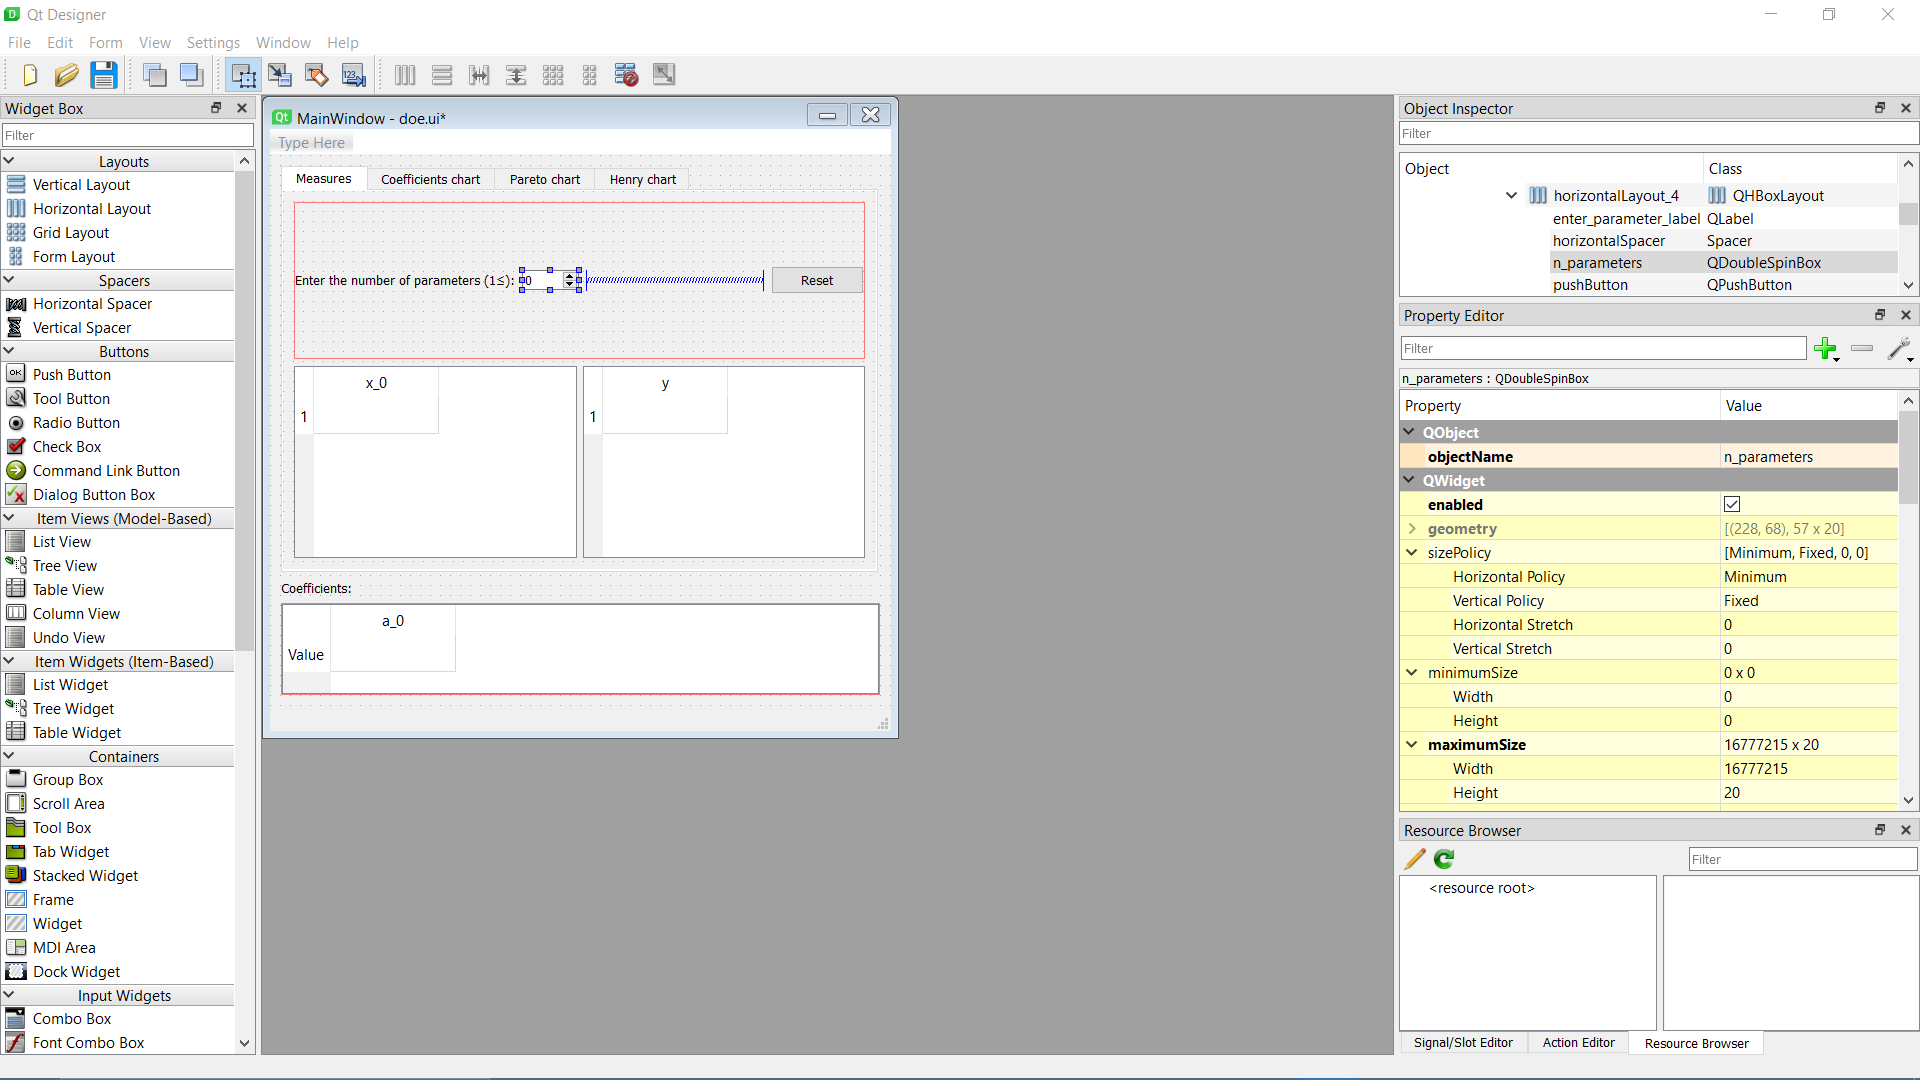
\includegraphics[width=\linewidth]{full_GUI}
\caption{Screen capture of the Qt Designer GUI\label{full_qt}}
\end{figure}

In the figure \ref{full_qt} the left panel the GUI element are available, and you can drop them in the application window. The Object inspector is on the right-side panel and allows you to browse through the different objects to change their parameters via the property editor.

N.B.: At the beginning of a project you can choose the kind of GUI you want to develop. Here, it is a \textquote{Main Window} application.

\clearpage
\subsubsection{Customised Widgets}
In this project by two times customized widgets have been used (using \pyv{mplwidget.py} and the \pyv{latexqtablewidget.py}). The first allows to use matplotlib to display charts and the second allows to render the header of the table widgets in LaTeX. To use them you must configure the widgets to use specify the class name and module name. It cannot be done after because you should not modify the generated Python script in the next step.

\begin{figure}[!ht]
\centering
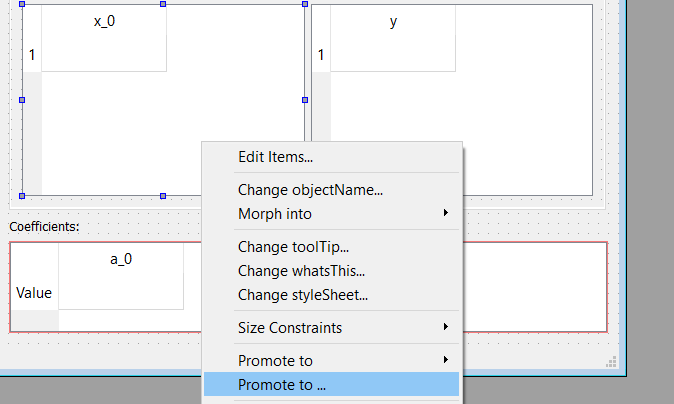
\includegraphics[width=0.8\linewidth]{promote_widget}
\caption{Promote the QTableWidget\label{fig:promote_widget}}
\end{figure}

The first step (figure \ref{fig:promote_widget}) is to open the \textquote{Promoted Widgets} window. Here we are configuring a QTableWidget and we want to add the LaTeX rendering feature.

\begin{figure}[!ht]
\centering
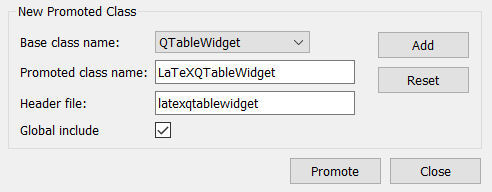
\includegraphics[width=0.6\linewidth]{config_promote}
\caption{Configure a customised QTableWidget\label{fig:config_promote}}
\end{figure}

The second step (figure \ref{fig:config_promote}) is to configure the new widgets by selecting the right base widget. Then by specifying the class name (it can be found in the header/module file of your customised widget class). And then to specify the header name without extension.

\subsubsection{Add the signals and slots}
By pressing the F4 key you can Add Signals/Slots to the objects. Personally, I do not use that part of the tools and I had manually the Signals and Slots in the third step.

Do not forget to save you project (as often as possible). Save all the scripts in the same source folder.

\subsection{Second step: Generate the Python script for the GUI}
We are using another Qt module to convert the .ui file generated by the Qt Designer tool. This tool will generate a Python code that will allow to create our specific layout created before. This tool is used in the \textquote{UI2PYconverter.py} script and the content of the script is the following.

\begin{pyverbatim}
# −∗− coding: utf−8 −∗−
''' PyQt5 uic module convert ui file (XML code) into py file (Python code) '''
from PyQt5 import uic

with open('doe.ui', 'r') as fin:
    with open('Uidoe.py', 'w') as fout:
        uic.compileUi(fin, fout, execute=True)
\end{pyverbatim}

The script will simply convert the \textquote{doe.ui} file to the \textquote{Uidoe.py} file. You should never modify directly the Python generated file since if you want to change the GUI layout a new script will be generated.

N.B.: The first line is there to specify to the interpreter the kind of encoding used for the Python script (this is not important).

\subsection{Third step: Create the main code}
Now that we have the GUI code, we want to bind it with behaviours and to link signals or events to it. You will write this script in a file with a .pyw extension (it will launch the script in windowed mode, without console).

\subsubsection{Minimal code}
The \textquote{base code} for my application is the following:
\begin{pyverbatim}[][breaklines]
# Import PyQt Widgets for PyQt5 version
import sys
from PyQt5.QtWidgets import QApplication, QMainWindow, QTableWidgetItem, QHeaderView
# Import pyqtSlot to connect sliders and DoubleSpinBox signals
from PyQt5.QtCore import pyqtSlot, Qt
# Import QIcon
from PyQt5.QtGui import QIcon
# Import Ui_MainWindow class from UiMainApp.py generated by uic module
from Uidoe import Ui_Design
# Import os
import os

class MainApp(QMainWindow, Ui_Design):
    """
    MainApp class inherit from QMainWindow and from
    Ui_MainWindow class in UiMainApp module.
    """

    def __init__(self):
        """Constructor or the initializer"""
        QMainWindow.__init__(self)
        # It is imperative to call self.setupUi (self) for the interface to initialize.
        # This is defined in Uidoe.py file automatically
        self.setupUi(self)
        self.setWindowTitle("Design of Experiments - by Vincent STRAGIER")
        

if __name__ == "__main__":
    # For Windows set AppID to add an Icon in the taskbar
    # https://stackoverflow.com/questions/1551605/how-to-set-applications-taskbar-icon-in-windows-7
    if sys.platform == 'win32':
        import ctypes
        from ctypes import wintypes
        appid = u'vincent_stragier.umons.doe.v1.0.0'  # arbitrary string
        ctypes.windll.shell32.SetCurrentProcessExplicitAppUserModelID(appid)

        lpBuffer = wintypes.LPWSTR()
        AppUserModelID = ctypes.windll.shell32.GetCurrentProcessExplicitAppUserModelID
        AppUserModelID(ctypes.cast(ctypes.byref(lpBuffer), wintypes.LPWSTR))
        appid = lpBuffer.value
        ctypes.windll.kernel32.LocalFree(lpBuffer)
    
    app = QApplication(sys.argv)
    # Launch the main app.
    MyApplication = MainApp()
    MyApplication.show()  # Show the form
    icon_path = os.path.join(os.path.dirname(sys.argv[0]), 'ico', 'fpms.svg')
    app.setWindowIcon(QIcon(icon_path))
    MyApplication.setWindowIcon(QIcon(icon_path))
    sys.exit(app.exec_())  # Execute the app
\end{pyverbatim}

This code will only display the GUI with a specific title and an icon (one on the window and one in the taskbar). In Windows you must use that kind of trick to display the logo. Notice the use of a .svg file that allows lossless scaling and transparency (alpha layer).


\subsubsection{Signals and slots}
To be able to get the inputs of the user, the signals of the objects must be connected to slots functions.

First add the signal connection in the \pyv{def __init__(self):} function definition of the \pyc{MainApp} class:

\begin{pyverbatim}
self.<objecName>.<signal>.connect(self.foo)
\end{pyverbatim}

where:

\begin{description}
\item[objectName] is the name of the specific object (set by default in Qt Designer or by you)
\item[signal] is the specific signal you want to connect (you must look through the documentation)
\item[foo] is the function that will be triggered by the connected signal.
\end{description}

Second you have to define the foo function as a member of the \pyc{MainApp} class by taking into account which arguments the signal will pass to foo:

% @pyqtSlot(<type>)
\begin{pyverbatim}
def foo(self, <type>:arg):
	pass
\end{pyverbatim}
where:

\begin{description}
\item[type] is the data type of the argument passed to your function foo by the signal
\item[arg] is the argument that will be retrieved by the function foo
\end{description}

% The @ symbol is there to use the function as a decorator of \pyv{pystSlot}.

Another method exists to handle the signals, using specific function names already linked to the signals. But the previous exposed method is easier and clearer.

\subsubsection{Interact with the GUI}
You can also use other methods to interact with the elements of you GUI. Mostly to change some value, to update a text, set default value or current value of some object, etc. There is plenty information on the internet about those methods.

\chapter{How to use the GUI}
% Link to the video and step to step tutorial
To use the GUI, you can look at my demonstration of the GUI on Youtube (\url{https://youtu.be/2I9Mx7gjNnI}).

The first step is to install Python and all the required Python modules (see the previous chapters).

The second step is to download the code from GitHub (\url{https://github.com/2010019970909/design_of_experiments}).

The third step is to start the \pyv{GUI_doe.pyw} script (figure \ref{fig:doe_gui}).

The fourth step is to set the number of parameters. Then to fill the $y$ column with your measurements (figure \ref{fig:doe_gui_filled}).

Now you can select any chart in the tabs (figure \ref{fig:doe_gui_coef}, figure, \ref{fig:doe_gui_pareto}, or figure \ref{fig:doe_gui_henry}) and the coefficients are displayed in the bottom of the GUI. If you want to reset the $y$ column you can use the reset button. Also, you can enter mathematical expression (not only values) in the cells, i.e., $5*pi*e**3$.

\begin{figure}[!ht]
\centering
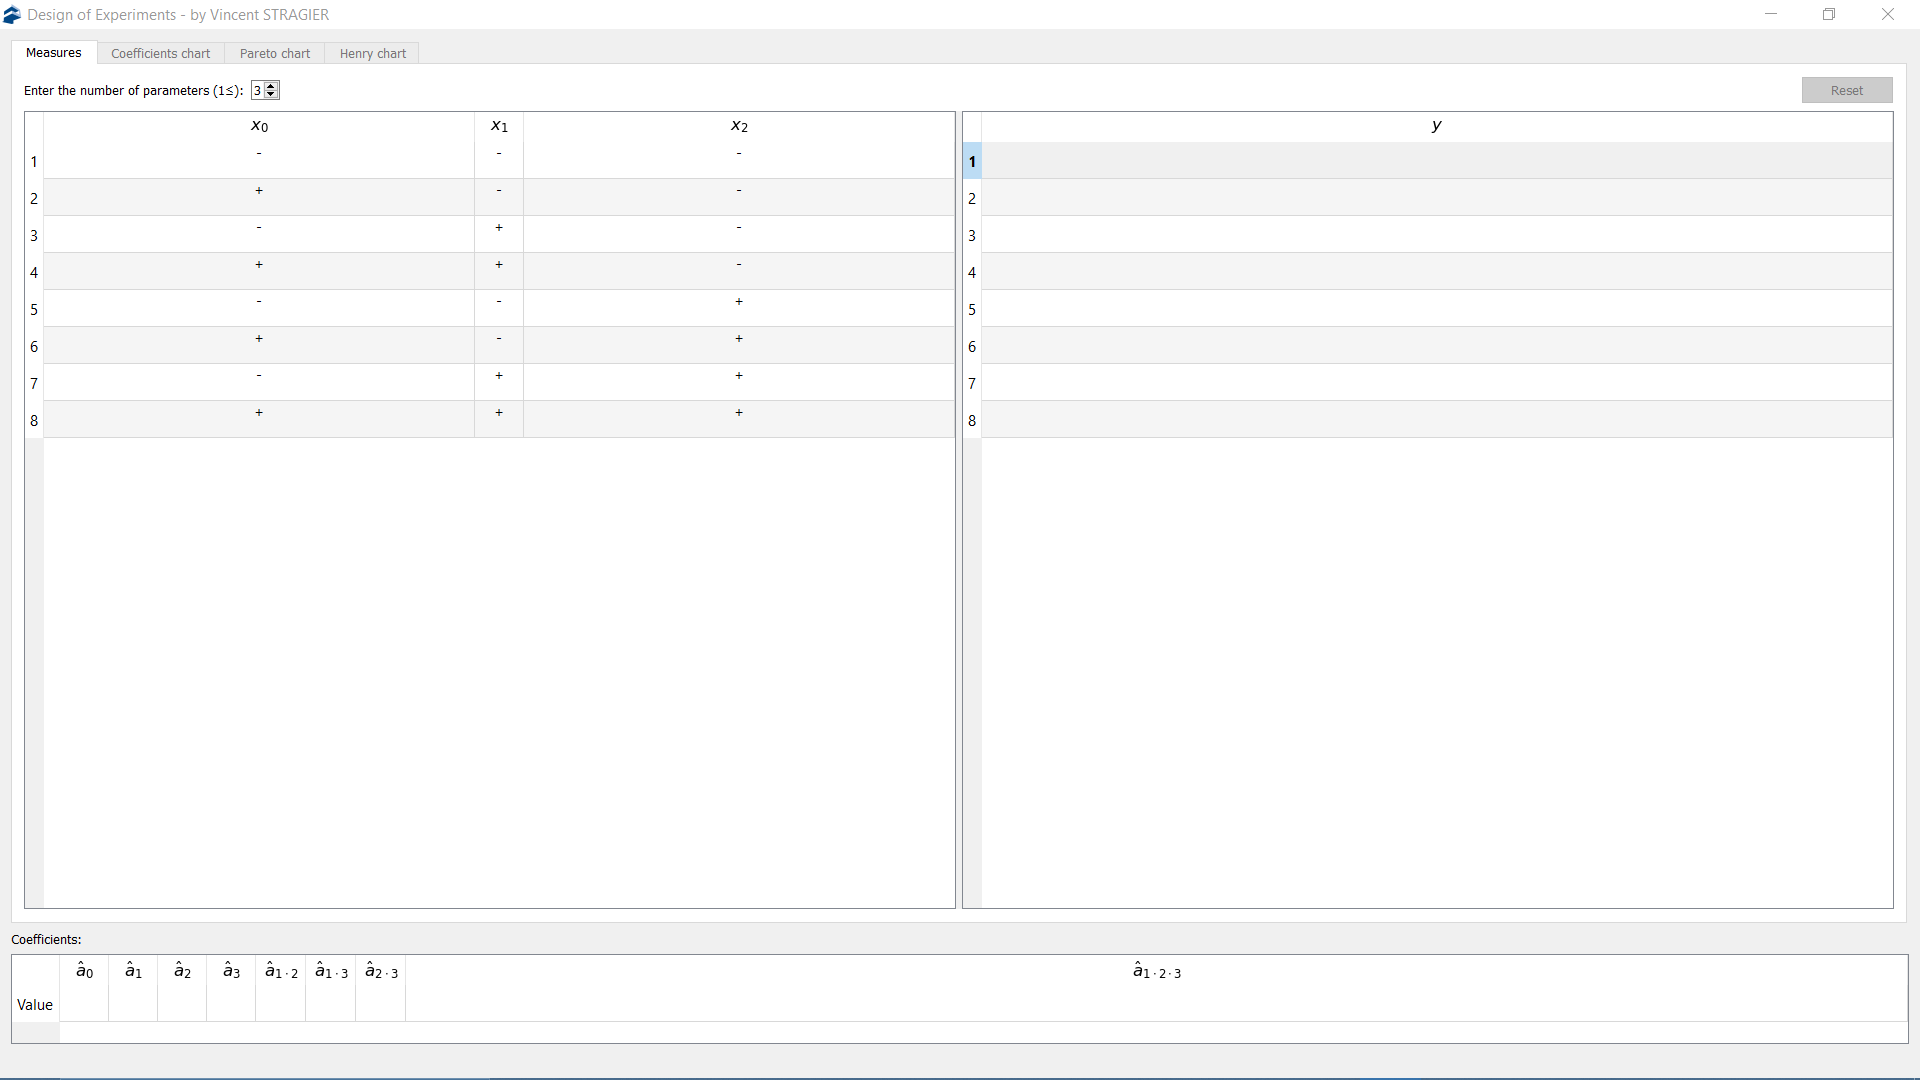
\includegraphics[width=\linewidth]{doe_gui}
\caption{DoE GUI\label{fig:doe_gui}}
\end{figure}

\begin{figure}[!ht]
\centering
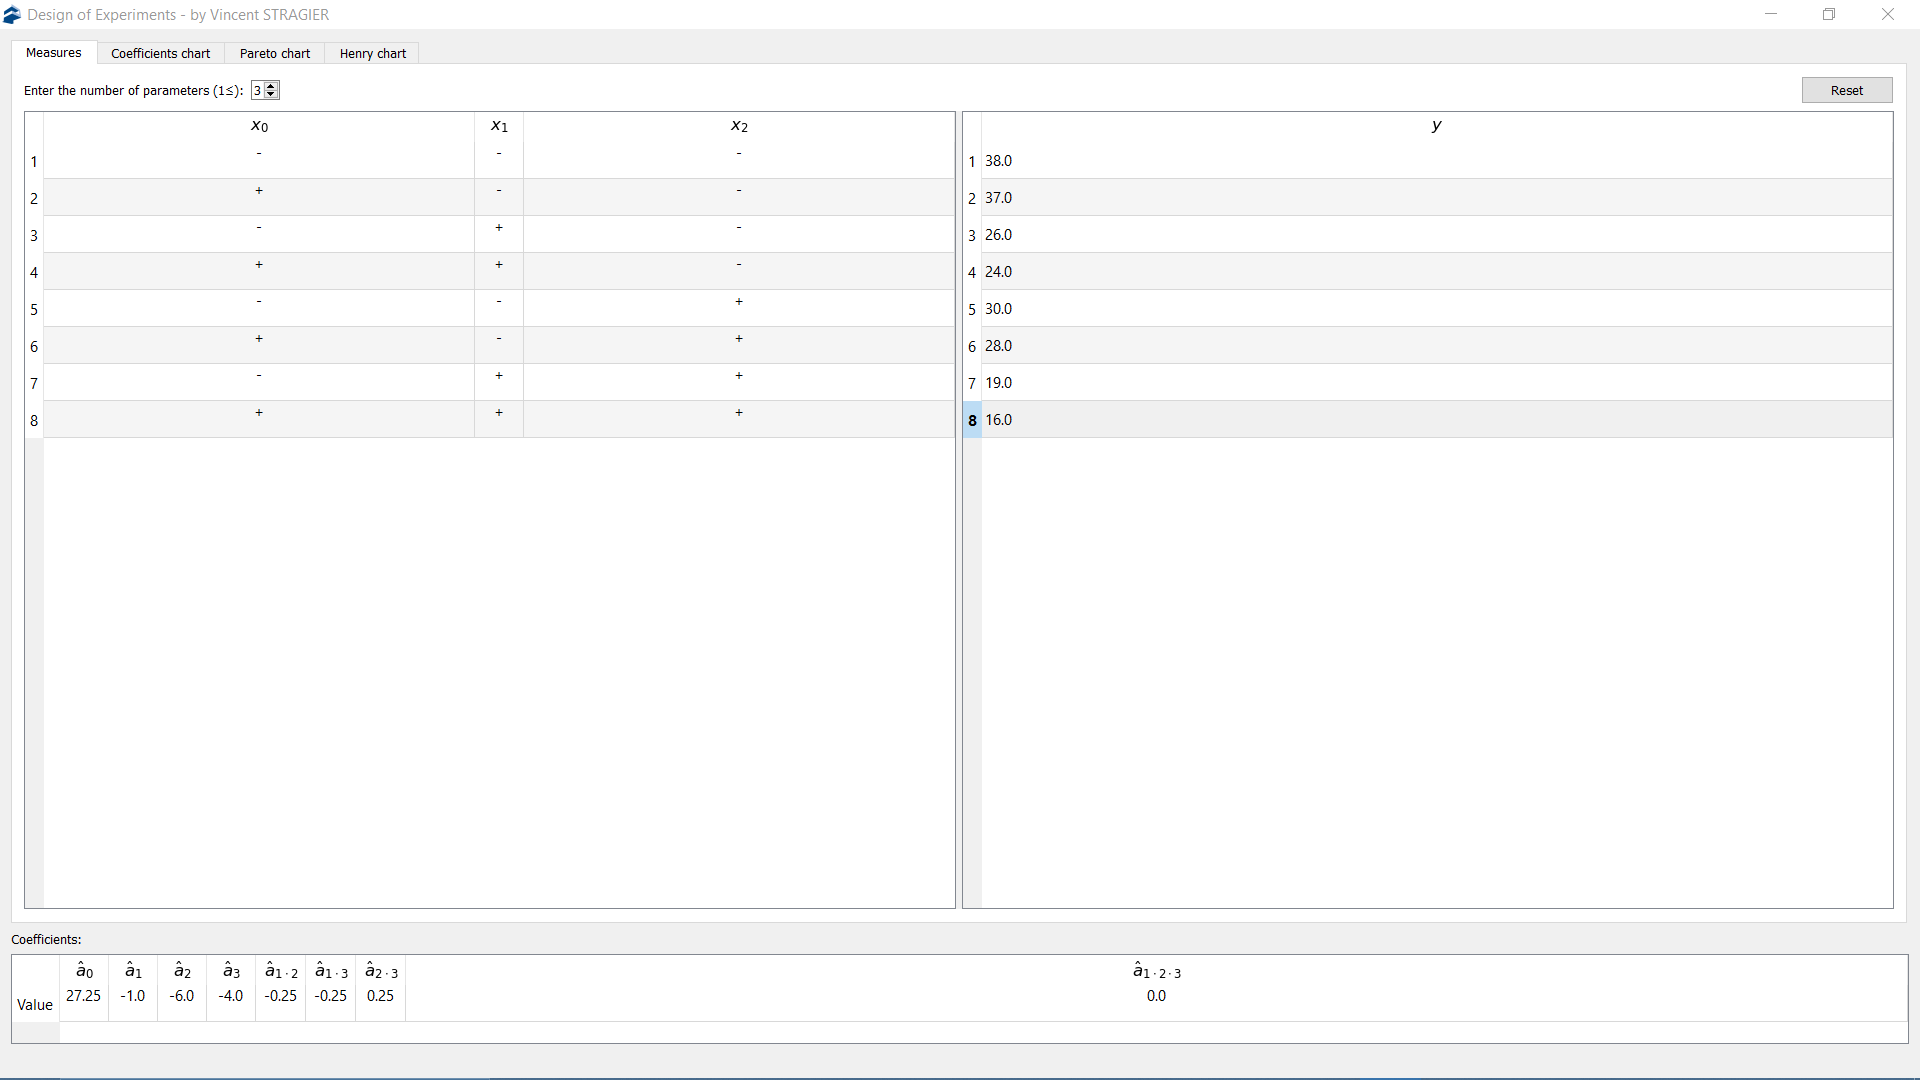
\includegraphics[width=\linewidth]{doe_gui_filled}
\caption{DoE GUI - Bitumen emulsion example\cite{goupy_methods_1993}\label{fig:doe_gui_filled}}
\end{figure}

\begin{figure}[!ht]
\centering
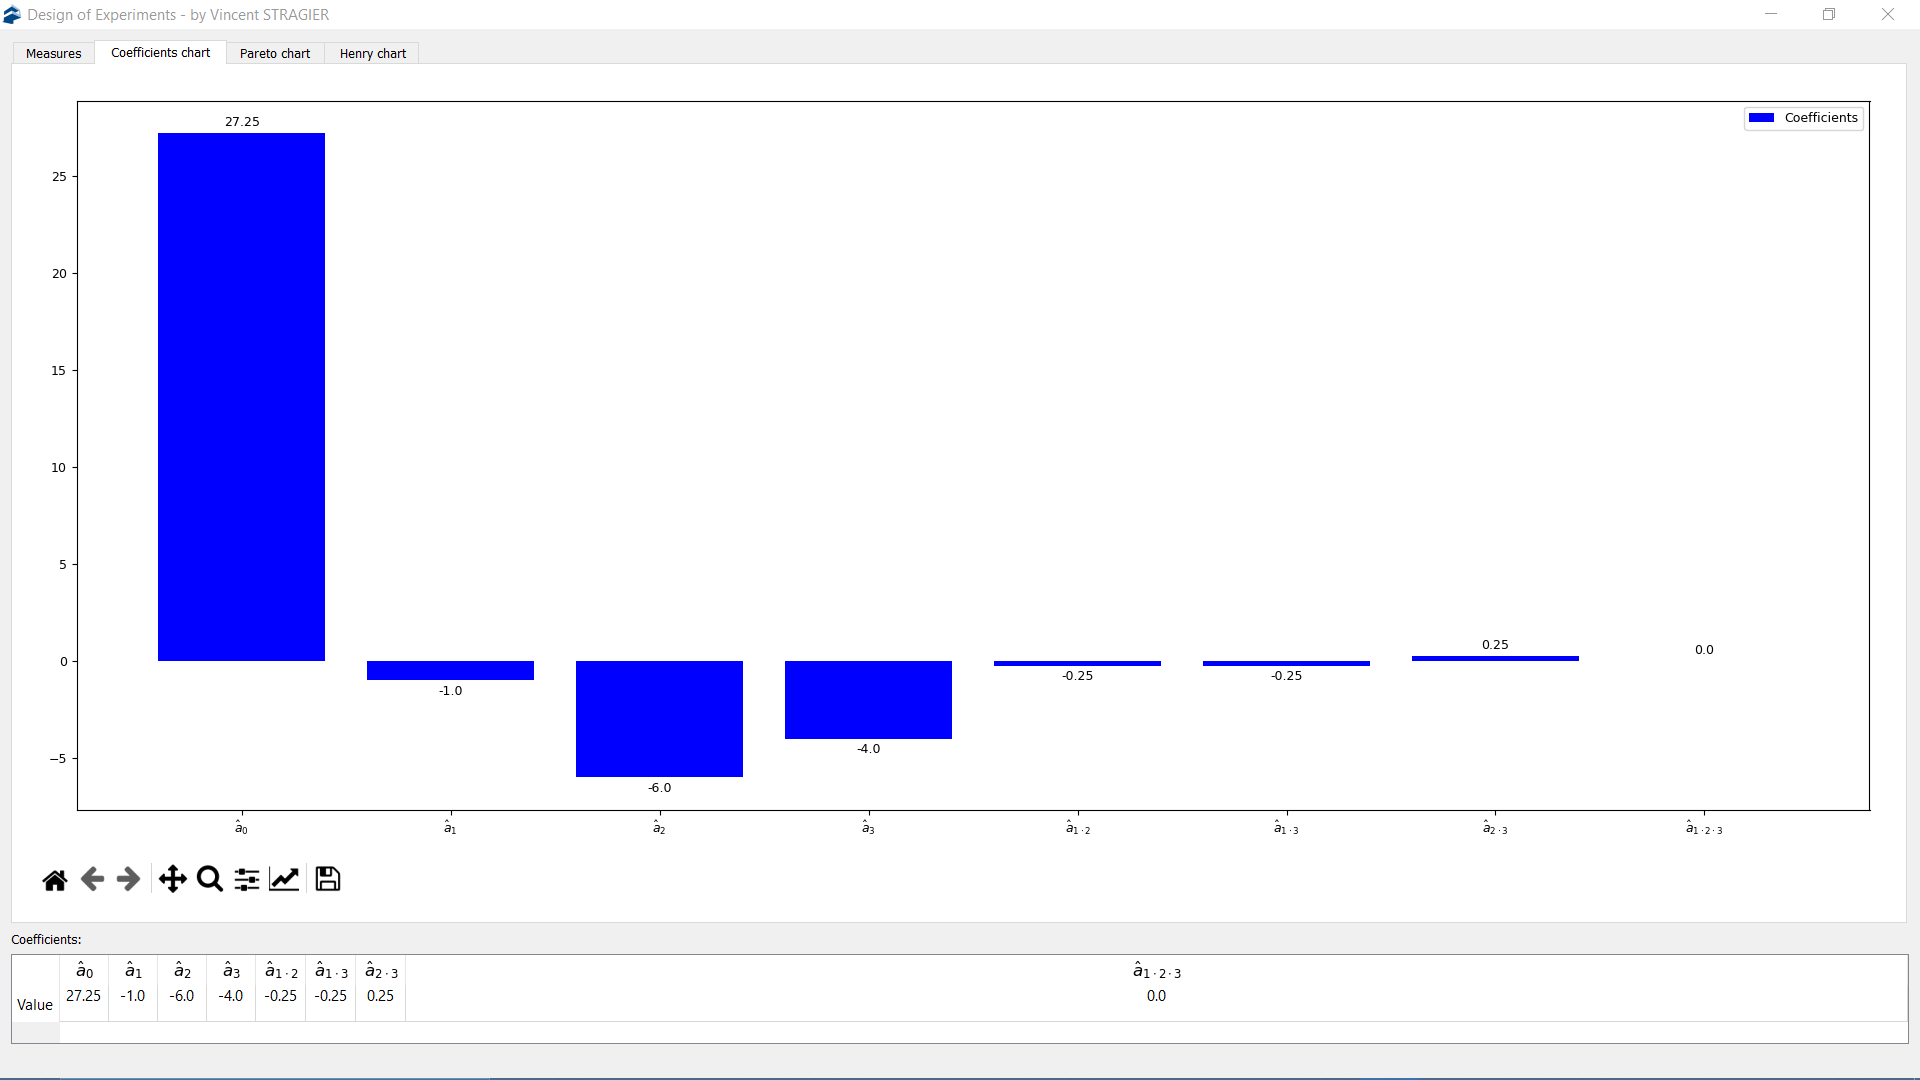
\includegraphics[width=\linewidth]{doe_gui_coef}
\caption{DoE GUI - Coefficient chart\label{fig:doe_gui_coef}}
\end{figure}

\begin{figure}[!ht]
\centering
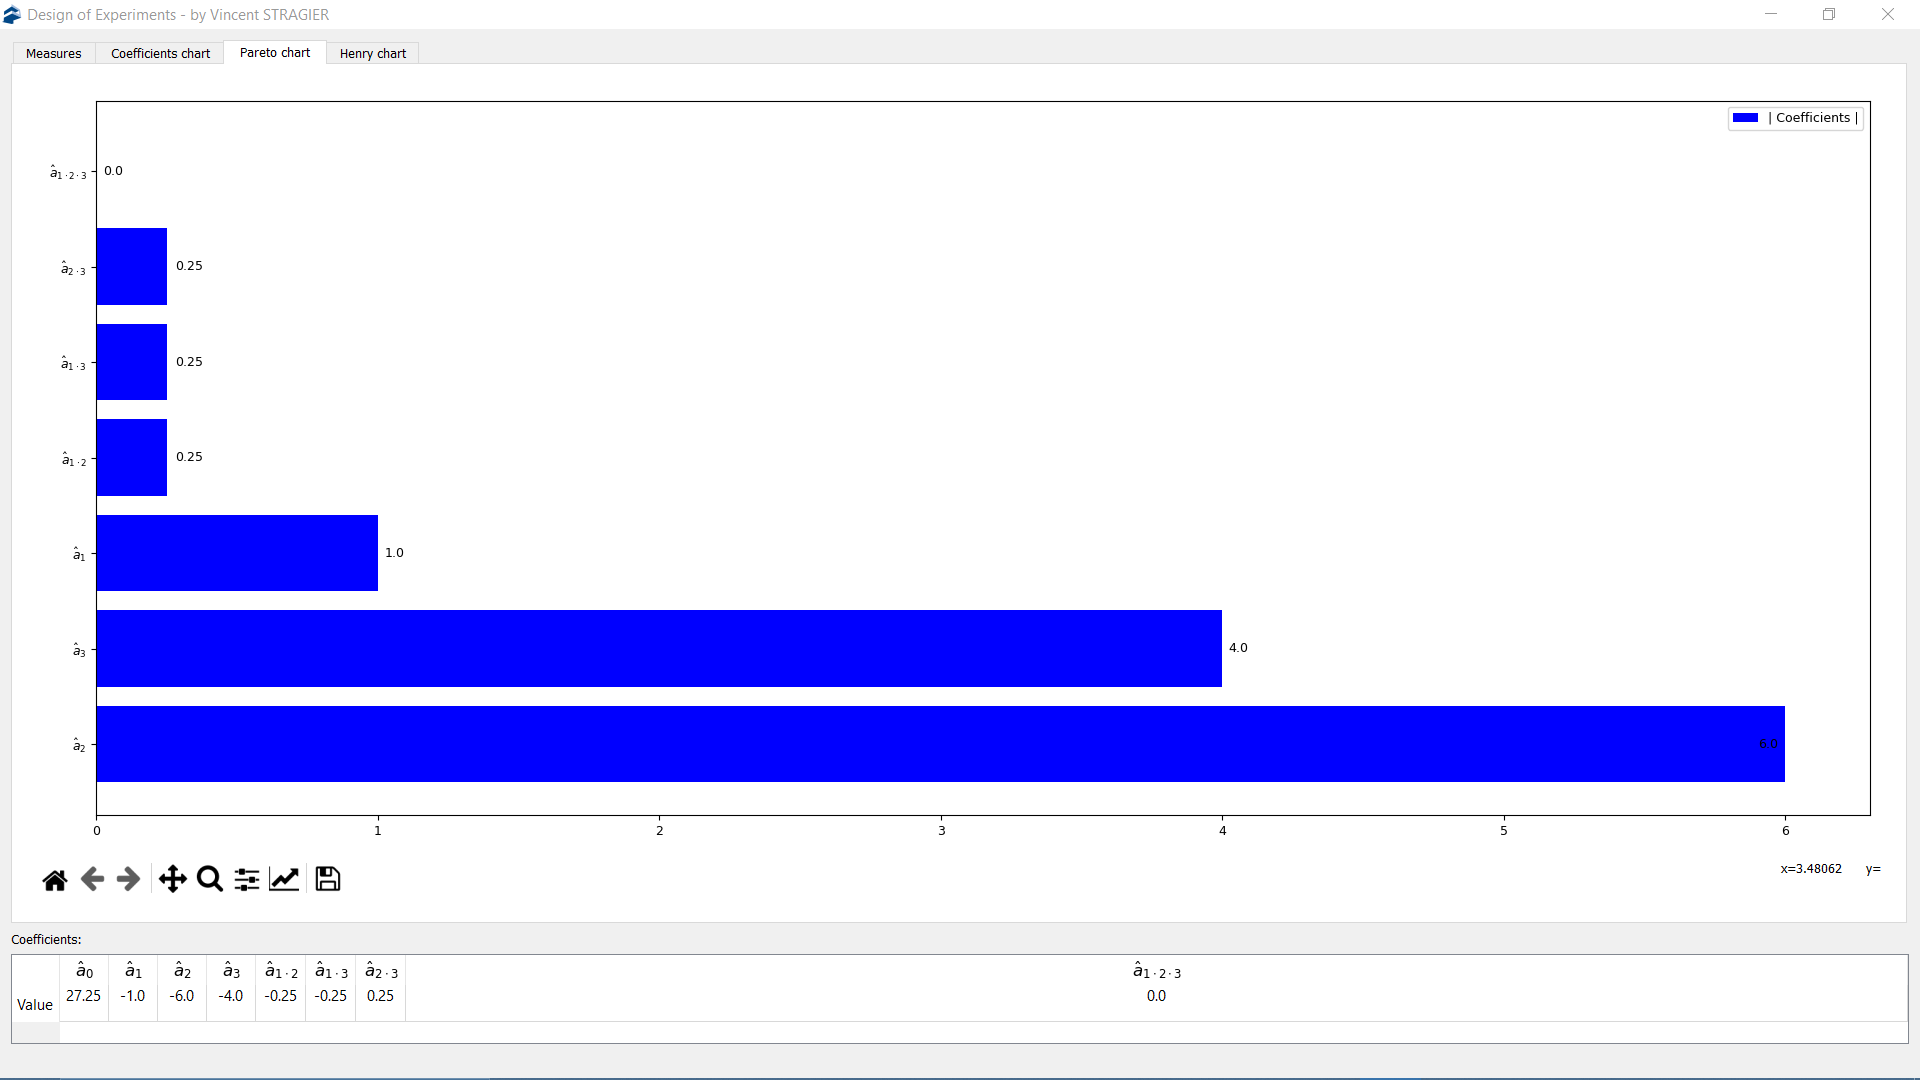
\includegraphics[width=\linewidth]{doe_gui_pareto}
\caption{DoE GUI - Pareto chart\label{fig:doe_gui_pareto}}
\end{figure}

\begin{figure}[!ht]
\centering
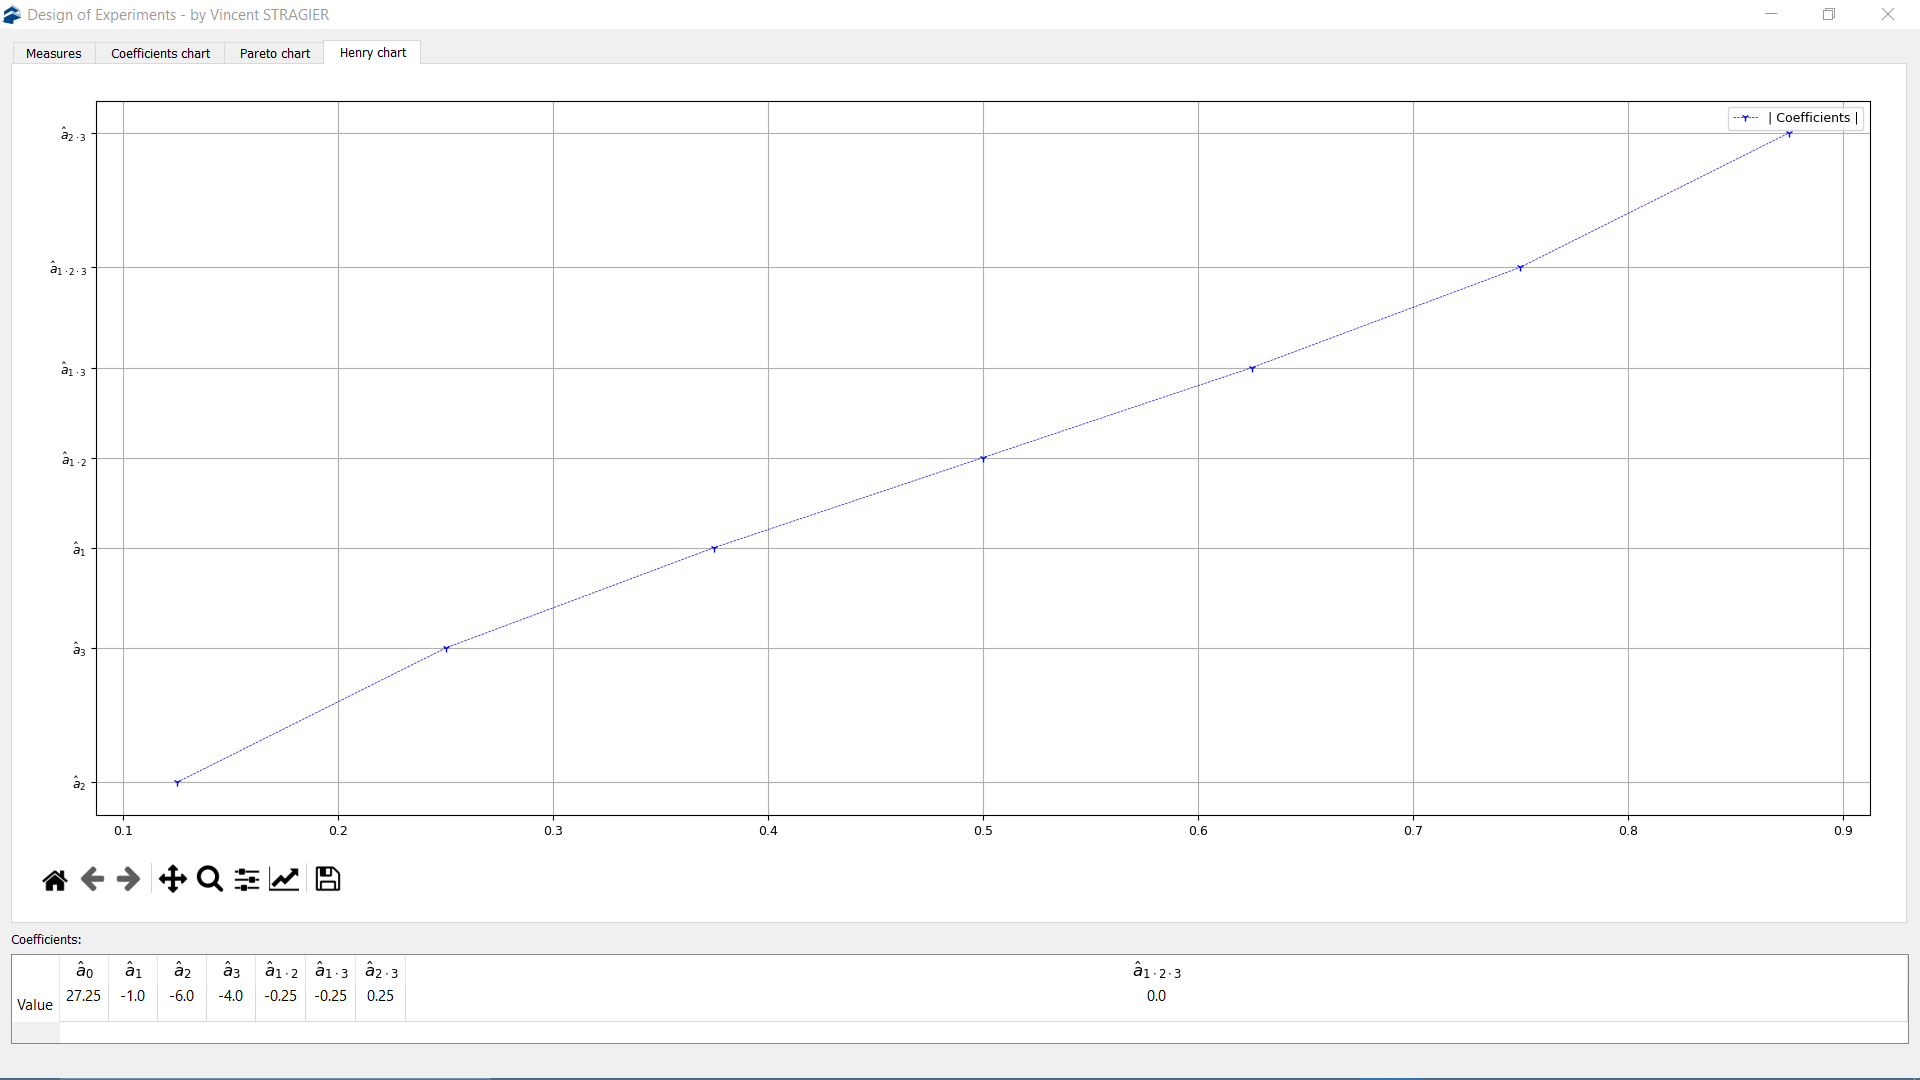
\includegraphics[width=\linewidth]{doe_gui_henry}
\caption{DoE GUI - Henry chart\label{fig:doe_gui_henry}}
\end{figure}

\phantomsection
\chapter*{Conclusion and analysis}
\addcontentsline{toc}{chapter}{Conclusion}

This program is working but could be improved. The computing time can be quite long to render the charts. However, each time the GUI or even the module implemented have been tested, the results were close (with sometime a light rounding error) to the solution of the examples. More charts could be added. The layout could be improved (stretching methods, etc.). The number of measured parameters could be increased. The file import, export could be improved (to select the file separators, the column(s) and line(s) to use, etc.).

%\nocite{*}
\printbibliography
\end{document}
